% Options for packages loaded elsewhere
\PassOptionsToPackage{unicode}{hyperref}
\PassOptionsToPackage{hyphens}{url}
\PassOptionsToPackage{dvipsnames,svgnames*,x11names*}{xcolor}
%
\documentclass[
  11pt,
]{article}
\usepackage{amsmath,amssymb}
\usepackage{lmodern}
\usepackage{ifxetex,ifluatex}
\ifnum 0\ifxetex 1\fi\ifluatex 1\fi=0 % if pdftex
  \usepackage[T1]{fontenc}
  \usepackage[utf8]{inputenc}
  \usepackage{textcomp} % provide euro and other symbols
\else % if luatex or xetex
  \usepackage{unicode-math}
  \defaultfontfeatures{Scale=MatchLowercase}
  \defaultfontfeatures[\rmfamily]{Ligatures=TeX,Scale=1}
\fi
% Use upquote if available, for straight quotes in verbatim environments
\IfFileExists{upquote.sty}{\usepackage{upquote}}{}
\IfFileExists{microtype.sty}{% use microtype if available
  \usepackage[]{microtype}
  \UseMicrotypeSet[protrusion]{basicmath} % disable protrusion for tt fonts
}{}
\makeatletter
\@ifundefined{KOMAClassName}{% if non-KOMA class
  \IfFileExists{parskip.sty}{%
    \usepackage{parskip}
  }{% else
    \setlength{\parindent}{0pt}
    \setlength{\parskip}{6pt plus 2pt minus 1pt}}
}{% if KOMA class
  \KOMAoptions{parskip=half}}
\makeatother
\usepackage{xcolor}
\IfFileExists{xurl.sty}{\usepackage{xurl}}{} % add URL line breaks if available
\IfFileExists{bookmark.sty}{\usepackage{bookmark}}{\usepackage{hyperref}}
\hypersetup{
  colorlinks=true,
  linkcolor=Maroon,
  filecolor=Maroon,
  citecolor=Blue,
  urlcolor=blue,
  pdfcreator={LaTeX via pandoc}}
\urlstyle{same} % disable monospaced font for URLs
\usepackage[margin=1in]{geometry}
\usepackage{graphicx}
\makeatletter
\def\maxwidth{\ifdim\Gin@nat@width>\linewidth\linewidth\else\Gin@nat@width\fi}
\def\maxheight{\ifdim\Gin@nat@height>\textheight\textheight\else\Gin@nat@height\fi}
\makeatother
% Scale images if necessary, so that they will not overflow the page
% margins by default, and it is still possible to overwrite the defaults
% using explicit options in \includegraphics[width, height, ...]{}
\setkeys{Gin}{width=\maxwidth,height=\maxheight,keepaspectratio}
% Set default figure placement to htbp
\makeatletter
\def\fps@figure{htbp}
\makeatother
\setlength{\emergencystretch}{3em} % prevent overfull lines
\providecommand{\tightlist}{%
  \setlength{\itemsep}{0pt}\setlength{\parskip}{0pt}}
\setcounter{secnumdepth}{-\maxdimen} % remove section numbering
\usepackage{setspace}
\usepackage{float}
\usepackage{mathtools}
\usepackage{natbib}
\usepackage[linesnumbered,ruled,vlined]{algorithm2e}
\setcitestyle{numbers,square,comma}
\usepackage{verbatim}
\usepackage{amsthm}
\usepackage{comment}
\ifluatex
  \usepackage{selnolig}  % disable illegal ligatures
\fi
\usepackage[]{natbib}
\bibliographystyle{plainnat}

\title{Clustering of Distributions on 1-Dimensional Manifolds}
\author{}
\date{\vspace{-2.5em}}

\begin{document}
\maketitle

\newcommand{\diag}{\mathrm{diag}}
\newcommand{\tr}{\mathrm{Tr}}
\newcommand{\blockdiag}{\mathrm{blockdiag}}
\newcommand{\indep}{\stackrel{\mathrm{ind}}{\sim}}
\newcommand{\iid}{\stackrel{\mathrm{iid}}{\sim}}
\newcommand{\Bernoulli}{\mathrm{Bernoulli}}
\newcommand{\Betadist}{\mathrm{Beta}}
\newcommand{\Uniform}{\mathrm{Uniform}}
\newcommand{\BG}{\mathrm{BernoulliGraph}}
\newcommand{\Categorical}{\mathrm{Categorical}}
\newcommand{\Multinomial}{\mathrm{Multinomial}}
\newcommand{\RDPG}{\mathrm{RDPG}}
\newcommand{\GRDPG}{\mathrm{GRDPG}}
\newtheorem{definition}{Definition}
\newtheorem{theorem}{Theorem}
\newtheorem{lemma}{Lemma}
\theoremstyle{remark}
\newtheorem*{remark}{Remark}
\theoremstyle{example}
\newtheorem*{example}{Example}
\newcommand{\dd}{\mathrm{d}}
\newcommand{\as}{\stackrel{\mathrm{a.s.}}{\to}}

\hypertarget{setup}{%
\section{Setup}\label{setup}}

Suppose we have two manifolds \(\mathcal{M}_1\) and \(\mathcal{M}_2\)
\(\in \mathbb{R}^d\), each of length 1, defined by \(f_1(t)\) and
\(f_2(t)\) respectively (\(f_k : [0, 1] \mapsto \mathbb{R}^d\)). Define
\(\delta\) as the minimum distance between any two manifolds, i.e.,
\(\delta = \max_{k, \ell} \min_{s, t} \|f_k(s) - f_\ell(t)\|\), and let
\(\delta > 0\). Restrict each \(f_k\) such that the distance along the
manifold between \(f_k(t)\) and \(f_k(s)\) is equal to the difference
between \(t\) and \(s\), i.e., \(f_k\) is the arclength parameterization
of \(\mathcal{M}_k\) (this also implies that each manifold is of length
1). Labels are sampled as
\(Z_1, ..., Z_n \stackrel{\mathrm{iid}}{\sim}\mathrm{Multinomial}(\alpha_1, \alpha_2)\),
and we define \(n_k\) as the number of labels with label \(k\). Sample
\(T_1, ..., T_n \stackrel{\mathrm{iid}}{\sim}F\) for some distribution
\(F\) with support \([0, 1]\). Finally, let \(X_i = f_{Z_i}(T_i)\) for
each \(i \in [n]\) be the latent vector of vertex \(i\), and gather the
latent vectors as
\(X = \begin{bmatrix} X_1 & \cdots & X_n \end{bmatrix}\). We observe
\(A \sim \mathrm{RDPG}(X)\) (or \(A \sim \mathrm{GRDPG}_{p,q}(X)\)) and
wish to recover \(Z_1, ..., Z_n\).

\hypertarget{preliminary-theory}{%
\section{Preliminary Theory}\label{preliminary-theory}}

\hypertarget{distributions-of-differences-of-order-statistics}{%
\subsection{Distributions of differences of order
statistics}\label{distributions-of-differences-of-order-statistics}}

Let \(D_i = X_{(i+1)} - X_{(i)}\). Then if \(\max_i D_i < \delta\), we
have sufficient separation of points in \(\mathcal{M}_1\). Then it is
sufficient to quantify \(P(\max_i D_i > \delta)\) as a function of \(n\)
and \(\delta\) and show that this converges to zero as \(n\) grows to
\(\infty\).

We denote \(f(x)\) as the density of each \(X_i\), \(g_i(x)\) as the
density of \(X_{(i)}\), \(g_{ij}(x, y)\) as the joint density of
\(X_{(i)}, X_{(j)}\), and \(h_i(d)\) as the density of \(D_i\) (with
corresponding capital letters for the cumulative distribution
functions).

The following are taken as given\footnote{\url{https://en.wikipedia.org/wiki/Order_statistic}}:

\begin{enumerate}
\def\labelenumi{\arabic{enumi}.}
\tightlist
\item
  \(g_i(x) = \frac{n!}{(n-i)! (i-1)!} (F(x))^{i-1} (1 - F(x))^{n-i} f(x)\).
\item
  \(g_{ij}(x, y) = \frac{n!}{(i-1)! (j-i-1)! (n-j)!} (F(x))^{i-1} (F(y) - F(x))^{j-i-1} (1 - F(y))^{n-j} f(x) f(y)\).
\item
  By convolution,
  \(h_i(d) = \int_0^{1} g_{i, i+1} (x, x + d) \mathrm{d}x\).
\end{enumerate}

\begin{lemma}[The probability density function of $D_i$]
\begin{equation}
\label{eq:pdf}
h_i(d) = \int_0^{1-d} \frac{n!}{(i-1)! (n-i-1)!} (F(x))^{i-1} (1 - F(x+d))^{n-i-1} f(x) f(x+d) \mathrm{d}x 
\end{equation}
\end{lemma}

\begin{proof}
This is just a direct consequence of 2 and 3 under the given statements. 
We also note that because the support of $X_i$ is $[0, 1]$, 
the integral only needs to be evaluated from $0$ to $1 - d$ 
because of the $f(x+d)$ and $1 - F(x+d)$ terms.
\end{proof}

\begin{lemma}[The cumulative distribution function of $D_i$]

\begin{equation}
\label{eq:cdf}
P(D_i < \delta) = H_i(\delta) = 1 - \int_0^{1-\delta} \frac{n!}{(n-i)! (i-1)!} (F(x))^{i-1} (1 - F(x + \delta))^{n-i} f(x) \mathrm{d}x
\end{equation}
\end{lemma}

\begin{proof}
$$
\begin{aligned}
H_i(\delta) & = \int_x^{x+\delta} h_i(d) \mathrm{d}d \\
& = \int_x^{x+\delta} \int_0^{1} \frac{n!}{(i-1)! (n-i-1)!} ((F(x))^{i-1} (1 - F(x+d))^{n-i-1} f(x) f(x+d) \mathrm{d}x \mathrm{d}d \\
& = \int_0^{1} \frac{n!}{(i-1)! (n-i-1)!} (F(x))^{i-1} f(x) \int_x^{x+\delta} (1 - F(x+d))^{n-i-1} f(x+d) \mathrm{d}d \mathrm{d}x \\
& = \int_0^{1} \frac{n!}{(i-1)! (n-i-1)!} (F(x))^{i-1} f(x) \int_{F(x)}^{F(x+\delta)} (1 - u)^{n-i-1} \mathrm{d}u \mathrm{d}x \\
& = \int_0^{1} \frac{n!}{(i-1)! (n-i)!} (F(x))^{i-1} f(x) ((1 - F(x))^{n-i} - (1 - F(x + \delta))^{n-i}) \mathrm{d}x \\ 
& = \int_0^1 g_i(x) \mathrm{d}x - \int_0^1 \frac{n!}{(i-1)! (n-i)!} (F(x))^{i-1} (1 - F(x + \delta))^{n-i} f(x) \mathrm{d}x \\
& = 1 - \int_0^1 \frac{n!}{(i-1)! (n-i)!} (F(x))^{i-1} (1 - F(x + \delta))^{n-i} f(x) \mathrm{d}x \\
\end{aligned}
$$

Because of the $x + \delta$ term, we can't actually evaluate this integral all the way up to $1$, and so we are left with 
$$
\begin{aligned}
& = 1 - \int_0^{1 - \delta} \frac{n!}{(i-1)! (n-i)!} (F(x))^{i-1} (1 - F(x + \delta))^{n-i} f(x) \mathrm{d}x.
\end{aligned}
$$
\end{proof}

\hypertarget{uniform-case}{%
\subsection{Uniform case}\label{uniform-case}}

\begin{lemma}[Differences between order statistics of a uniform distribution]
If $X_1, ..., X_n \stackrel{\mathrm{iid}}{\sim}\mathrm{Uniform}(0, 1)$, then each $D_i \sim \mathrm{Beta}(1, n)$.
\end{lemma}

\begin{proof}
We begin with Eq. (\ref{eq:pdf}), plugging in $f(x) = 1$ and $F(x) = x$:

$$
h_i(d) = \int_0^{1-d} \frac{n!}{(i-1)! (n-i-1)!} x^{i-1} (1-x-d)^{n-i-1} \mathrm{d}x
$$

Then we proceed with integration by parts, setting 
$u = x^{i-1} \implies du = (i-1) x^{i-2}$ and 
$dv = (1-x-d)^{n-i-1} dx \implies v = -\frac{1}{n-i} (1-x-d)^{n-i-1}$. 
Note that $u v |_0^{1-d} = 0$ in this case. This yields

$$
= \frac{n!}{(i-1)! (n-i-1)!} \int \frac{i-1}{n-i} x^{i-2} (1-x-d)^{n-i} \mathrm{d}x
$$

Then applying integration by parts again until the $x^p$ term disappears, we get:

$$
\begin{aligned}
& = \frac{n!}{(i-1)! (n-i-1)!} \frac{(i-1)!}{(n-i) \cdots (n-2)} \int_0^{1-d} (1-x-d)^{n-2} \mathrm{d}x \\
& = -\frac{n (n-1)}{n-1} (1-x-d)^{n-1} \Big|_0^{1-d} \\
& = n (1 - d)^{n-1}
\end{aligned}
$$

This the density function for $\mathrm{Beta}(1, n)$, completing the proof.
\end{proof}

\begin{theorem}
Let $X_1, ..., X_n \stackrel{\mathrm{iid}}{\sim}\mathrm{Uniform}(0, 1)$. 
Then for any $\epsilon$ and $\delta > 0$, 
there exists an $N = O \big(\frac{-\log \epsilon}{\delta} \big)$ such that 
$P(\max_i X_{(i+1)} - X_{(i)} < \delta) \geq 1 - \epsilon$ when $n > N$.
\end{theorem}

\begin{proof}[Proof (sketch)]
Since $X_{(i+1)} - X_{(i)} = D_i \sim \mathrm{Beta}(1, n)$, 
$P(X_{(i+1)} - X_{(i)} < \delta) = 1 - (1 - \delta)^n $. This yields

$$
\begin{aligned}
P(\max_i D_i < \delta) & \geq (P(D_i < \delta))^{n-1} \\
& = (1 - (1 - \delta)^n)^{n-1} \\
& \approx e^{-n \exp(-n \delta)}.
\end{aligned}
$$

In the limit $n \to \infty$, this goes to 1.
\end{proof}

\hypertarget{test-for-intersecting-manifolds}{%
\subsubsection{Test for intersecting
manifolds}\label{test-for-intersecting-manifolds}}

\begin{theorem}
Let $\mathcal{M}_1$ and $\mathcal{M}_2$ be two one-dimensional manifolds of unit length with $n / 2$ points drawn uniformly along each manifold.

Suppose we want to perform a hypothesis test for whether the ends of the manifolds meet. 
The $H_0$ is the case where $\delta = 0$ and $H_1$ is the case where $\delta > 0$. 
We define the test statistic $T_n$ as follows: 
Construct an $\epsilon$-neighborhood graph using the smallest $\epsilon$ required to make the graph connected. 
Let $\{d_i\}$ be the set of edge lengths of this graph. 
Define $T_n = \max_i d_i$. 
Then $T_n / 2 \stackrel{d}{\to} \mathrm{Beta}(1, n)$ under $H_0$. 
\end{theorem}

This theorem isn't 100\% correct---in reality, we want to draw edges
along the ``super-manifold'' that is created by joining the two
manifolds (under \(H_0\)). But if \(H_0\) is true, then these lengths
should converge to the true distances along the super-manifold.

\hypertarget{community-detection-for-non-affine-one-dimensional-manifolds}{%
\subsubsection{Community detection for ``non-affine'' one-dimensional
manifolds}\label{community-detection-for-non-affine-one-dimensional-manifolds}}

For non-intersecting manifolds, distance-based graph techniques provide
a straightforward method for community detection. However, this is not
the case in many models with community structure. For example, the
latent structure that induces the degree-corrected block model consists
of line segments that emanate from the origin, so each community is a
one-dimensional subspace, or linear manifold, and these manifolds meet
at the origin. For the DCBM, a straightforward approach to community
detection involves an ASE followed by clustering based on angles (e.g.,
cosine similarity). As an extension to this case, we consider community
detection for two one-dimensional manifolds that meet at the origin.

The method that is proposed is as follows:

\begin{enumerate}
\def\labelenumi{\arabic{enumi}.}
\tightlist
\item
  For each point \(x_i\), compute \(\|x_i\|\).
\item
  Construct an \(\epsilon\)-neighborhood graph for \(X\), choosing
  \(\epsilon\) large enough that the graph is connected. Alternatively,
  construct a \(K\)-NN graph, again, choosing \(K\) so that the graph is
  connected.
\item
  Remove the vertex \(v_j\) that corresponds to the point
  \(x_j = \min_i \|x_i\|\). If this results in two disconnected
  subgraphs, we are done. Otherwise, continue removing vertices in
  ascending order of magnitude until the graph is disconnected. Then map
  each component to a community.
\item
  Estimate curves for each community (e.g., using polynomial
  regression). Map each removed point to a community based on its
  distance to the curve.
\end{enumerate}

In the following example, we draw \(64\) points each uniformly along two
manifolds in \(\mathbb{R}^2\) that intersect at the origin:

\begin{center}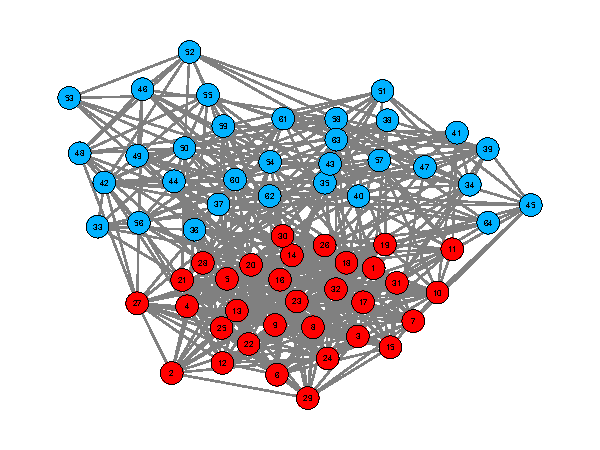
\includegraphics{distributions-on-1d-manifolds_files/figure-latex/unnamed-chunk-2-1} \end{center}

The \(5\)-NN graph is as follows:

\begin{center}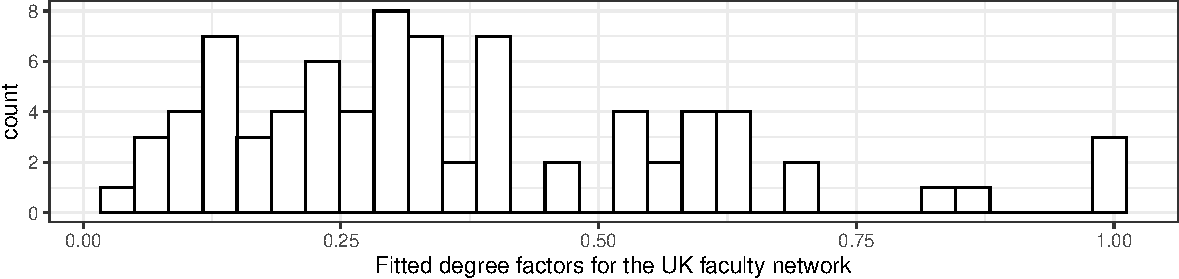
\includegraphics{distributions-on-1d-manifolds_files/figure-latex/unnamed-chunk-3-1} \end{center}

Removing the 10 points closest to the origin results in the following:

\begin{center}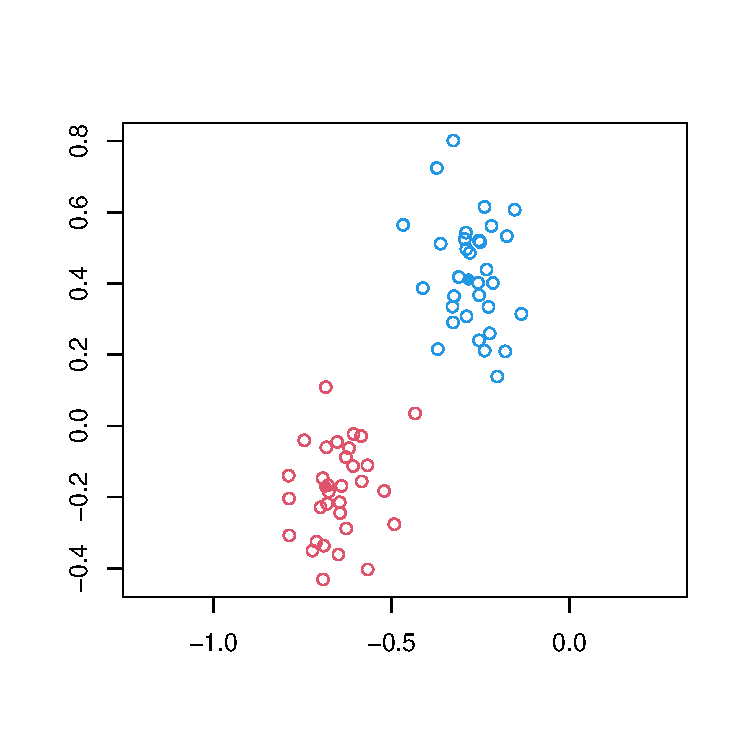
\includegraphics{distributions-on-1d-manifolds_files/figure-latex/unnamed-chunk-5-1} \end{center}

\hypertarget{general-case}{%
\subsection{General case}\label{general-case}}

\begin{theorem}
\label{thm:generalized}
Let $X_1, ..., X_n \stackrel{\mathrm{iid}}{\sim}F$ with support $[0, 1]$, and suppose $f(x)$ is continuous and $f(x) \geq a > 0$ everywhere on the support. 
Let $D_i = X_{(i+1)} - X_{(i)}$. 
Then for any $\epsilon > 0$, there exists $N \in \mathbb{N}$ such that $P(\max_i D_i < \delta) \geq 1 - \epsilon$ when $n > N$.
\end{theorem}

\begin{proof}[Proof (sketch)]
We start with Eq. (\ref{eq:cdf}):

$$P(D_i \leq \delta) = 1 - \int_0^{1-\delta} \frac{n!}{(n-i)! (i-1)!} (F(x))^{i-1} (1 - F(x + \delta))^{n-i} f(x) \mathrm{d}x.$$

Making the approximation $F(x+\delta) \approx F(x) + \delta f(x)$ 
and bounding $f(x) \geq a$, we get:

$$P(D_i \leq \delta) \geq 1 - \int_0^{1-\delta} \frac{n!}{(n-i)! (i-1)!} (F(x))^{i-1} (1 - F(x) - a \delta)^{n-i} f(x) \mathrm{d}x.$$

Then making the substitution $u = F(x) \implies du = f(x) \mathrm{d}x$, we obtain 

$$1 - \int_0^{F(1-\delta)} \frac{n!}{(n-i)! (i-1)!} u^{i-1} (1 - u - a \delta)^{n-i} \mathrm{d}u$$

Evaluating the integral yields

$$P(D_i < \delta) = 1 - (1 - a \delta)^n + (1 - F(1-\delta) - a \delta)^n.$$

Then as before,

$$
\begin{aligned}
P(\max_i D_i < \delta) & = P(\text{all } D_i < \delta) \\
& = 1 - P(\text{some } D_i > \delta) \\
& \geq 1 - \sum_i^{n-1} P(D_i > \delta) \\
& = 1 - (n - 1) (1 - a \delta)^n + (n - 1) (1 - F(1 - \delta) - a \delta)^n
\end{aligned}
$$

This converges to $1$ in the limit $n \to \infty$.

We can also approximate $F(1 - \delta) \approx 1 - a \delta$, which yields 
$1 - (n - 1) (1 - a \delta)^n$. Setting this $\geq 1 - \epsilon$ ...
\end{proof}

\hypertarget{extension-to-multidimensional-manifolds}{%
\subsection{Extension to multidimensional
manifolds}\label{extension-to-multidimensional-manifolds}}

Here, we extend the results on the line to the unit hypercube. The
following theorem is a direct consequence of Lemma 2 of
\citet{trosset2020rehabilitating}.

\begin{theorem}
\label{thm:multidim}
Let $X_1, ..., X_n \stackrel{\mathrm{iid}}{\sim}F$ with support $[0, 1]^r$, and $f(x) \geq a > 0$ everywhere on the support. 
Define $E_n$ as the event that an $\eta$-neighborhood graph constructed from the sample is connected. 
Then for any $\epsilon > 0$, there exists $N = O \bigg( \frac{\log \epsilon \eta^r / r^{r/2}}{\log (1 - \frac{a \eta^r}{r^{r / 2}})} \bigg)$ such that $P(E_n) > 1 - \epsilon$ when $n \geq N$.
\end{theorem}

\begin{proof}[Proof (sketch)]
Divide the hypercube $[0, 1]^r$ into a grid of sub-hypercubes of side length at most $\eta / \sqrt{r}$. 
$E_n$ is satisfied if each sub-hypercube contains at least one $X_i$ from the sample. 

$$
\begin{aligned}
P(E_n) & = 1 - P(\text{some cells don't contain } X_i) \\
& \geq 1 - \sum_k^{\lceil \sqrt{r} / \eta \rceil^r} \prod_i^n P(X_i \text{ is not in the } k^{th} \text{ hypercube}) \\
& \geq 1 - \lceil \sqrt{r} / \eta \rceil^r (1 - a \eta^r / r^{r/2})^n
\end{aligned}
$$

Setting this $\geq 1 - \epsilon$ and solving for $n$ yields the desired rate. 
\end{proof}

\hypertarget{algorithms}{%
\section{Algorithms}\label{algorithms}}

TBD

\hypertarget{computational-results}{%
\section{Computational Results}\label{computational-results}}

TBD

\renewcommand\refname{References}
  \bibliography{misc.bib}

\end{document}
